\chapter{A broad overview of Amazon Web Services}
This is intended to give you some context about AWS.
It can give you the ability to build a platform which scales automatically with little to no running cost. That's the beauty of serverless. Startups could go and try out new ideas and if it didn't work, you could just stop and delete it. Without much collateral damage. No 3-5 yr contracts for renting servers.

\section{History}
AWS gave you Virtual Machines and then you could go in and terminate it. You didn't have to live with the collateral damage. 

In 2003, Chris Pinkham and Benjamin Black presented a paper on amazon's internal structure. This could become a business proposal which they presented.

\begin{itemize}
	\item SQS launched in 2004.
	\item AWS launched in 2006.
	\item all of Amazon.com moved to AWS in 2010.
	\item First re:Invent Conference in 2012.
	\item Certification launched in 2013.
	\item Committed to 100\% renewable energy for global footprint they wanted for 2014.
	\item AWS breaks out revenue: 6 Billion USD per annum and grew at 90\% a year.
	\item AWS re:Invent released a host of AI Services. Run rate hits $27$ Billion USD.
	\item AWS launched ML and AI certificates in 2019.
	\item Alexa specialty certificate in 2019.
\end{itemize}

AWS went for the developers first, instead of corporates, when it released. Dropbox, AirBnB started on AWS.

\section{A Brief Overview}
Services are grouped in A-Z. There are an awful lot of services. However, a lot of them are not very relevant to Certified Solutions Architect associate exam.
Let's talk about the relevant ones.

\subsection{High Level Services}
\begin{itemize}
	\item Compute
	\item Storage	
	\item Databases
	\item Migration and Transfer.
\end{itemize}

\section{AWS Global Infrastructure}
differences between regions and availability zone. Northern Virginia is the oldest region and all new services come out first on there. But also goes down the most (once a year), so don't deploy there. On top of global infrastructure sit the following services:
\begin{itemize}
	\item Compute. (EC2, Lambda etc.)
	\item Storage. Putting files into buckets. (S3).
	\item Databases. Relational Databases (RDS), Non-relational databases (Dynamo DB and RedShift).
	\item Migration and transfer. way of getting things to and from AWS (Snobble).
	\item Network and Content Delivery. VPCs, Cloud front (CDM).
	\item Developer Tools. (Covered in Developer associate exam).
	\item Robotics, Blockchain and Sattelite. (NR).
	\item Management and Governance, Media Services, Machine Learning (Some depth of ML is required). 
	\item Analytics.
	\item Security, Identity and Compliance.
	\item Mobile.
	\item AR and VR. (NR)
	\item Application Integration. (NR)
	\item AWS Cost Management.
	\item Customer Engagement.
	\item Business Applications.
	\item Desktop and App Streaming.
	\item IOT and Game Development.
\end{itemize}

\begin{figure}[htbp]
	\centering
	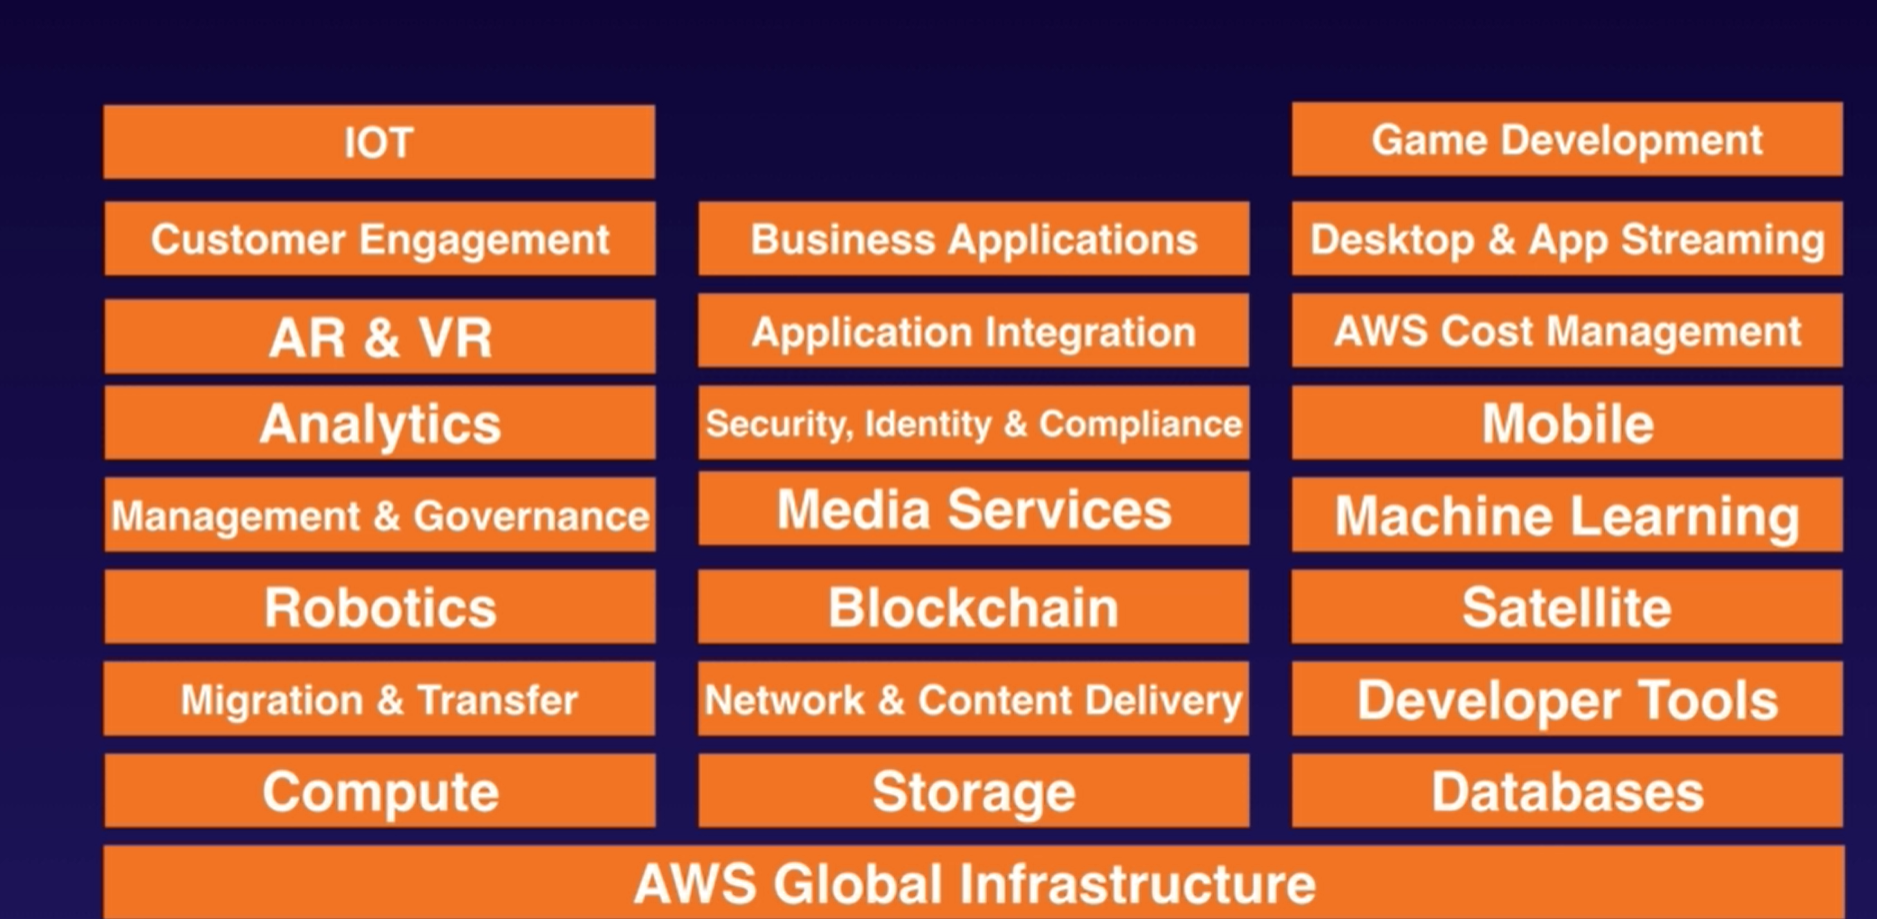
\includegraphics[width = 150mm]{./images/Most-services.png}
	\caption{Most services available as of 2019}
\end{figure}

\subsection{region and availability zone and edge location}
19 regions \& 57 availability zones in december 2018. 5 more regions and 15 more AZs in 2019. \\
\textbf{\textit{Availability Zones:}}
\begin{itemize}
	\item An availability zone is one/several close data center.
	\item Everything to do with cloud sits in data centers.
\end{itemize}

A \textbf{Region} is a simple distinct geographic area. Every region has 2, 3 or more availability zones. Always more \textit{edge locations than regions}. \textbf{Edge location} are end points for AWS for caching content in local zone. Someone from sydney requests a file from new york, they dl it from newyork. Now it will be cached in sydney edge location. for increased speed in the next dl. Typically consists of CloudFront, Amazon's CDN etc. Singapore, Osaka, Mumbai, region etc. Whole bunch of different edge locations as well.

In future will cover a few relevant services but not all of them. Ones we need to know:

\begin{figure}[htbp]
	\centering
	\subfloat[Need to Know services]{
	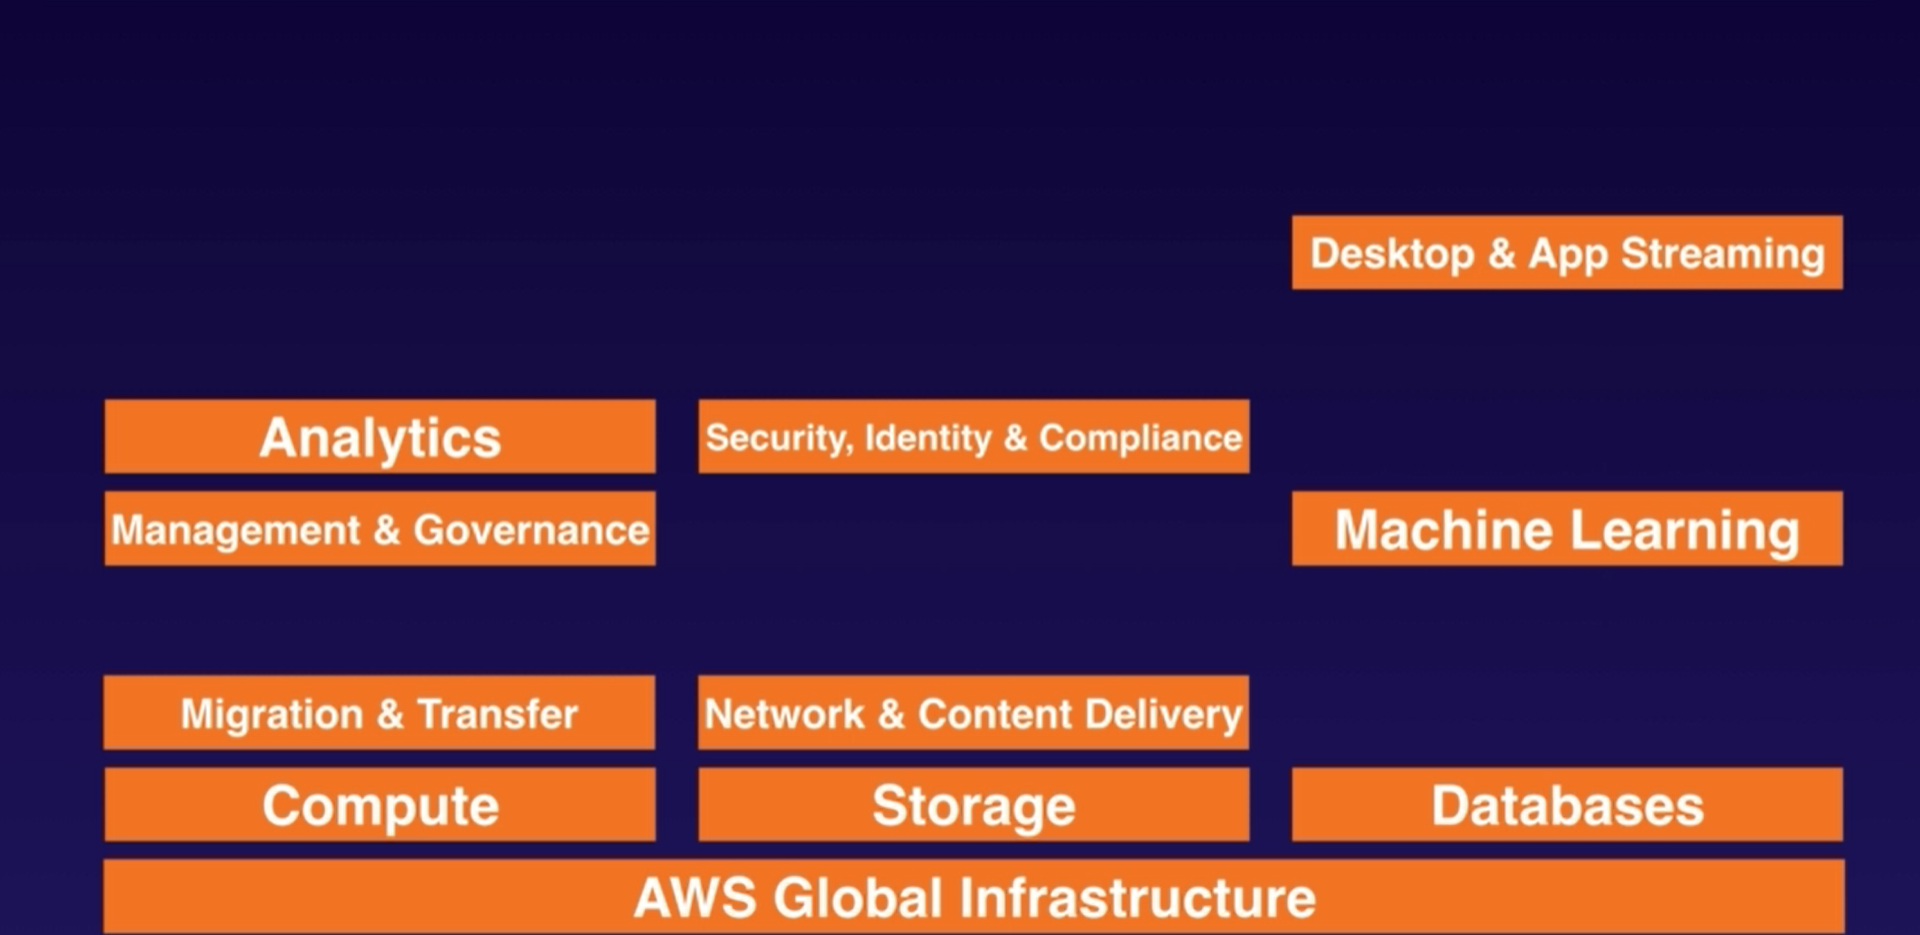
\includegraphics[width = 75mm]{./images/Need-to-Know-services.png}	
}
	\subfloat[Bread and butter services]{
	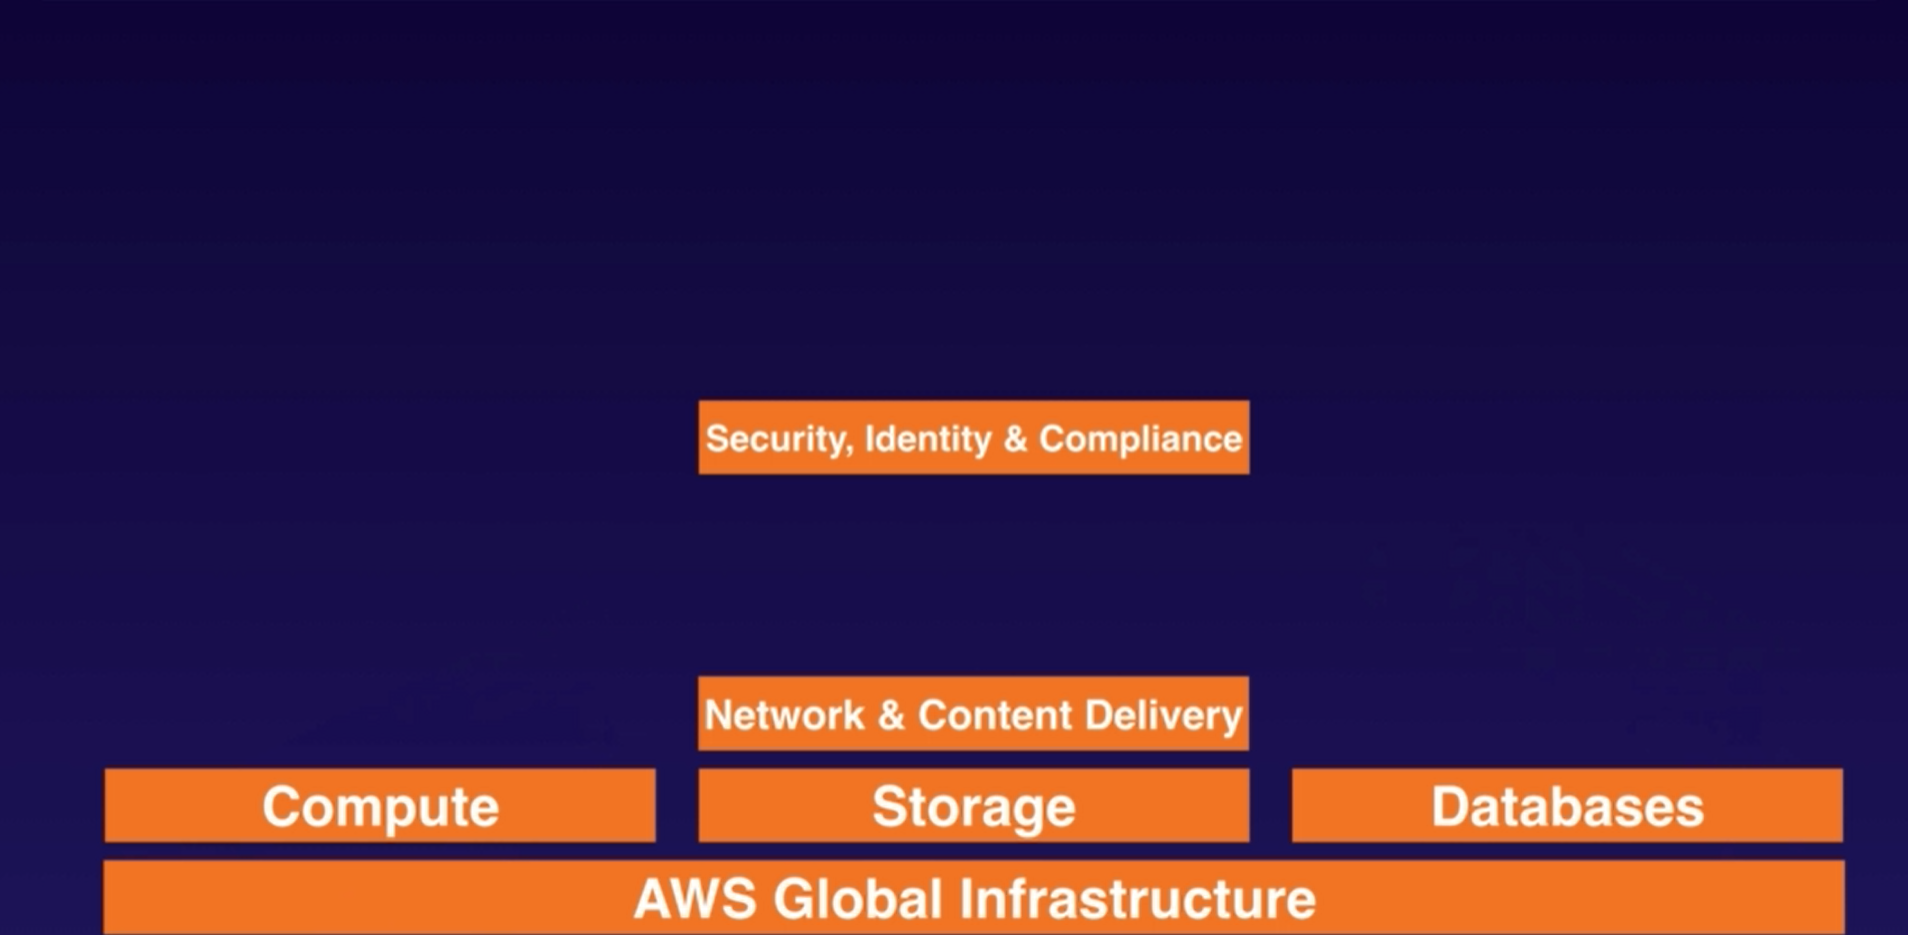
\includegraphics[width = 75mm]{./images/Core-services.png}	
}
	\caption{Services relevant to the exam}
\end{figure}

\section{Virtual Private Cloud}
A Virtual Private Cloud (VPC) is a virtual network dedicated to a single AWS account. It is logically isolated from other virtual networks in the AWS cloud, providing compute resources with security and robust networking functionality.

\section{summary concepts}
\begin{itemize}
	\item Regions: Distinct geographical locations holding multiple AZs.
	\item Availability Zones: One or two data centers holding all computers of AWS.
	\item Edge locations: Distinct end points used for caching content.
	\item Virtual Private Cloud: A private cloud within AWS dedicated to a particular account. It provides compute resources securely and robustly. Secure from other private clouds within AWS. 
\end{itemize}